% ===========================================================
% case_studies.tex
% ===========================================================
\section{Case Studies}
\label{sec:cases}

\subsection{Pedagogical IEEE 9-Bus Example}
\label{sec:cases-9bus}

The IEEE 9-bus system with the dispatch reported in
Table~\ref{tab:9bus-dispatch} is used to exercise the picker on a
synthetic case where the answer is unambiguous.  Three thermal
units are assumed dispatched: a hydro at $\$5$, a CCGT with two
tiers $(\$45, \$58)$, and a coal at $\$70$.  The system load is
chosen so that $\lambda^{\mathrm{CEN}}=\$58.0$/MWh.  Among the
dispatched-non-forced units the absolute-closest CV is the
\$58 CCGT tier, confirming the picker's selection.  At the slightly
lower system price $\lambda=\$56$/MWh the picker still selects
the same unit because the next-down CV (\$45) is further away in
absolute distance ($\$11$ vs.\ $\$2$).  Only when $\lambda$ falls
below $\$51.5$ does the picker switch to the $\$45$ tier.  The
implied $\hat\lambda$ has a regime-dependent step structure that
mirrors the SCVIC ladder of Fig.~\ref{fig:ladder}.

\begin{table}[h]
  \centering
  \caption{Pedagogical IEEE 9-bus dispatch and SCVIC ladder used
  in Section~\ref{sec:cases-9bus}.}
  \label{tab:9bus-dispatch}
  \begin{tabular}{lrrrrr}
    \toprule
    Unit & $\underline{p}$ & $\overline{p}$ & $p$ & $c$ &
    fuel \\
    & MW & MW & MW & \$/MWh & \\
    \midrule
    Hydro-A   & 0   & 80  & 60  & 5   & water \\
    CCGT-B-T1 & 50  & 100 & 100 & 45  & GNL \\
    CCGT-B-T2 & 100 & 250 & 220 & 58  & GNL \\
    Coal-C    & 100 & 200 & 0   & 70  & coal \\
    \bottomrule
  \end{tabular}
\end{table}

The pedagogical case clarifies one design choice: when the picker
encounters a forced unit (e.g.\ a take-or-pay GNL-CCGT cleared by
\texttt{consigna}=\texttt{CI}), the unit \emph{remains} a valid
candidate as long as it is operating interior to its bounds.  Only
forced-at-pmin units are dropped.  This is the operational
realisation of the rule that ``the next \SI{1}{\MWh} can come from
any unit with positive headroom and a finite ramp rate'', which
distinguishes the present picker from the strict
last-dispatched-cleared rule of \cite{SilerEvans2012}.

\subsection{Real CEN Application: 29 Buses on 2026-04-22}
\label{sec:cases-real}

The pipeline was run against the cached CEN snapshot for the
operating day 2026-04-22.  The bus catalogue
(Section~\ref{sec:bridge}) contains \num{29} reconciled production
buses spanning the north (CRUCERO~220, ESPERANZA~220), the
north-centre (D.ALMAGRO~110, GUACOLDA~220), the centre (ALTO
MELIPILLA~220, EL~SALTO~220, LOS~ALMENDROS~220), the centre-south
(ANCOA~220/500, ITAHUE~220), the south-centre (CHARRÚA~220,
ANTUCO~220, CONCEPCI\'ON~220), and \num{16} additional aggregated
backbone buses.  The full day yields \num{2494} (bus, quarter)
cells across \num{86} settled quarters (the early morning
\num{00}{:}\num{00}{-}\num{02}{:}\num{15} window is filled by the
\texttt{best\_real} cmg-online fallback policy).

Fig.~\ref{fig:lambda} reproduces the headline outcome.  Panel~A
plots the published $\lambda^{\mathrm{CEN}}$ for all \num{29} buses
overlaid by region (one colour per region) with the cross-bus
median in bold.  Panel~B plots the reconstructed $\hat\lambda$
under the same colour convention; the close visual agreement at
both the median and the per-bus dispersion is the qualitative
validation of the method.  Panel~C plots the per-bus absolute
error $|\hat\lambda - \lambda^{\mathrm{CEN}}|$, with the
P90 envelope shaded in grey.  The error is concentrated below
\$0.5/MWh for over \SI{90}{\percent} of cells.  The transient
spikes near hour~\num{6} and hour~\num{17} correspond to the
ramp-up/down of GNL CCGT units between SCVIC tiers — these are
precisely the cells flagged by the \texttt{tier\_uncertainty}
criterion of Section~\ref{sec:eps}.

\begin{figure*}[t]
  \centering
  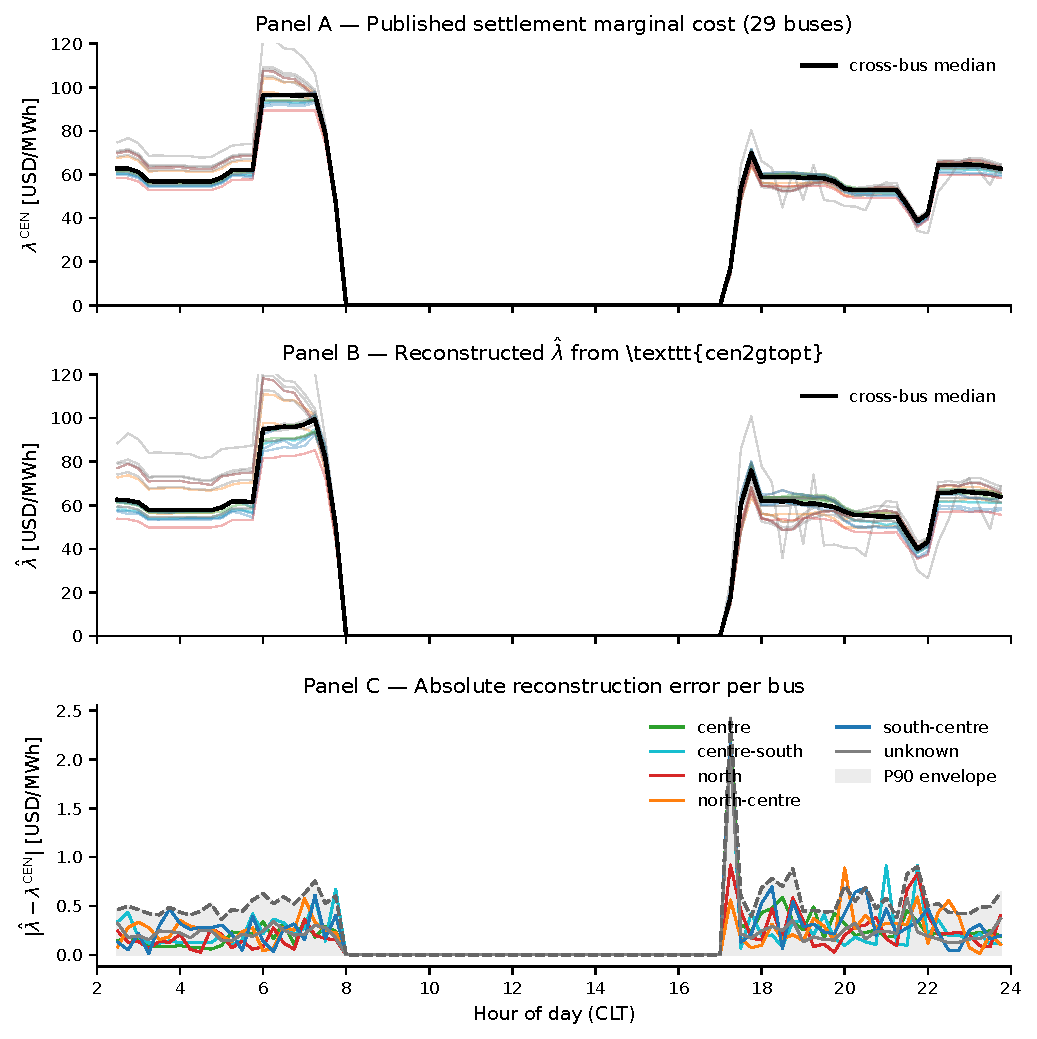
\includegraphics[width=\textwidth]{figures/fig_lambda_real_vs_reconstructed_2026_04_22.pdf}
  \caption{Headline reconstruction validation for 2026-04-22.
  \textbf{(A)} Published $\lambda^{\mathrm{CEN}}$ per bus, region-coloured;
  bold black is cross-bus median.  \textbf{(B)} Reconstructed
  $\hat\lambda$ from the pipeline.  \textbf{(C)} Absolute reconstruction
  error per bus, with the cross-bus median per region and the P90
  envelope.}
  \label{fig:lambda}
\end{figure*}

Fig.~\ref{fig:eps} shows the corresponding median bus marginal
emission factor $\varepsilon^{\mathrm{bus}}$.  The shaded band
along the bottom of the figure colour-codes the dominant marginal
fuel per quarter: GNL (orange) dominates the non-renewable hours,
biomass and water-marginal hours sit near zero, and a brief diesel
peak appears in the early evening.  The mid-day depression below
\SI{0.05}{\tonne\mathrm{CO}_2\per\MWh} reflects the
solar-curtailment regime where $\lambda^{\mathrm{CEN}}\le\$0.5$ and
the picker returns regime~$=$~\texttt{renewable\_curtailment} with
$\varepsilon=0$; this regime accounts for \num{1073} of the
\num{2494} cells (\SI{43.0}{\percent}).

\begin{figure}[t]
  \centering
  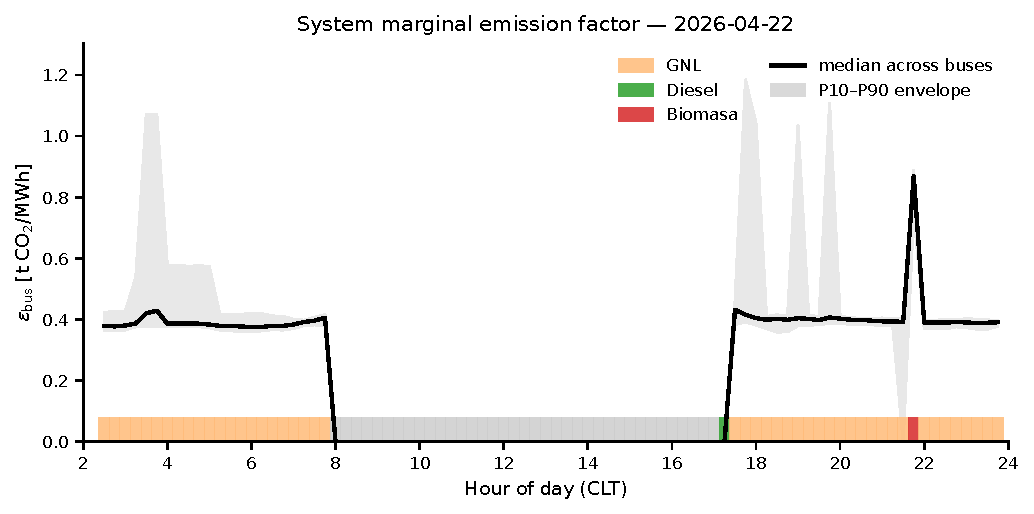
\includegraphics[width=\columnwidth]{figures/fig_marginal_emission_2026_04_22.pdf}
  \caption{System bus marginal emission factor for 2026-04-22.
  Solid black line: cross-bus median; grey band: P10–P90 envelope
  across buses.  The bottom strip colour-codes the dominant
  marginal fuel per quarter (GNL, biomass, diesel, etc.).}
  \label{fig:eps}
\end{figure}

Fig.~\ref{fig:coherence} is a diagnostic heatmap of the assigned
marginal-unit name per (bus, quarter).  By construction the picker
operates per island, so all buses sharing an island in the
quarter share the same marginal unit; what the heatmap therefore
visualises is the spatial extent of each marginal unit's island
across the day.  Across the \num{474} quarter-island cells, the
marginal-unit assignment is coherent in zero cases of
contradiction (\num{0}/\num{474}), confirming that the picker is
deterministic at the island level.

\begin{figure}[t]
  \centering
  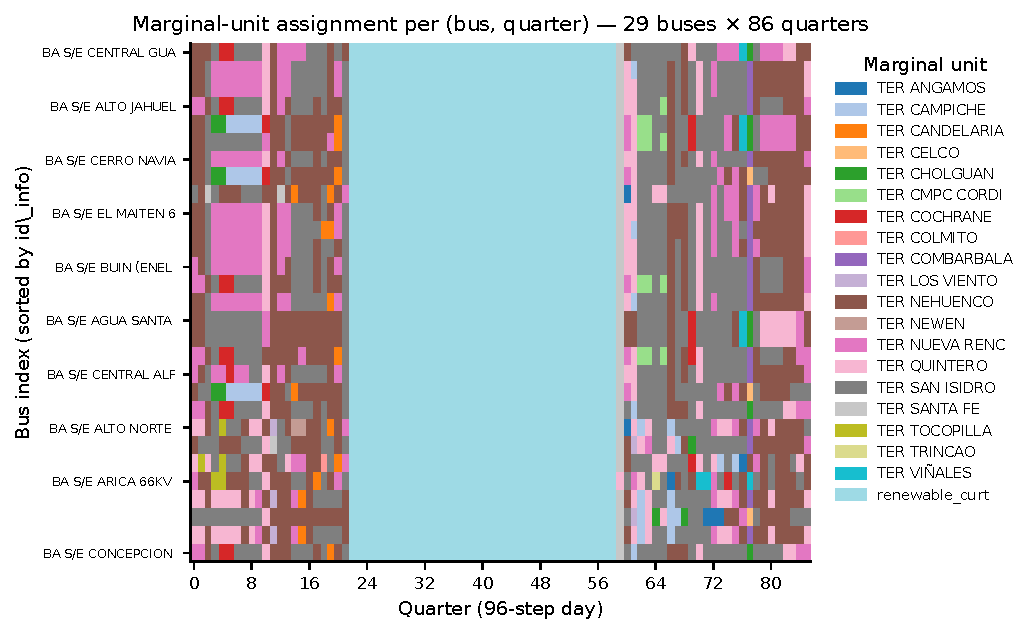
\includegraphics[width=\columnwidth]{figures/fig_per_island_coherence_heatmap.pdf}
  \caption{Marginal-unit assignment per (bus, quarter) for
  2026-04-22.  Rows are buses (sorted by \texttt{id\_info}),
  columns are 15-minute quarters.  Colour encodes the assigned
  marginal-unit name; horizontal bands indicate the spatial extent
  of each marginal unit's island.}
  \label{fig:coherence}
\end{figure}

Fig.~\ref{fig:region} disaggregates the absolute error by
region.  The centre-Santiago and north regions exhibit the
tightest tracking (mean $|\Delta|$ near $\$0.13$/MWh), the
centre-south and south-centre regions are slightly looser
(\$0.17–\$0.20/MWh), and the unknown-region buses (those whose
heuristic mapping did not classify into a named region) inherit a
mean of \$0.17/MWh.  No region exceeds a P90 of $\$0.61$/MWh.

\begin{figure}[t]
  \centering
  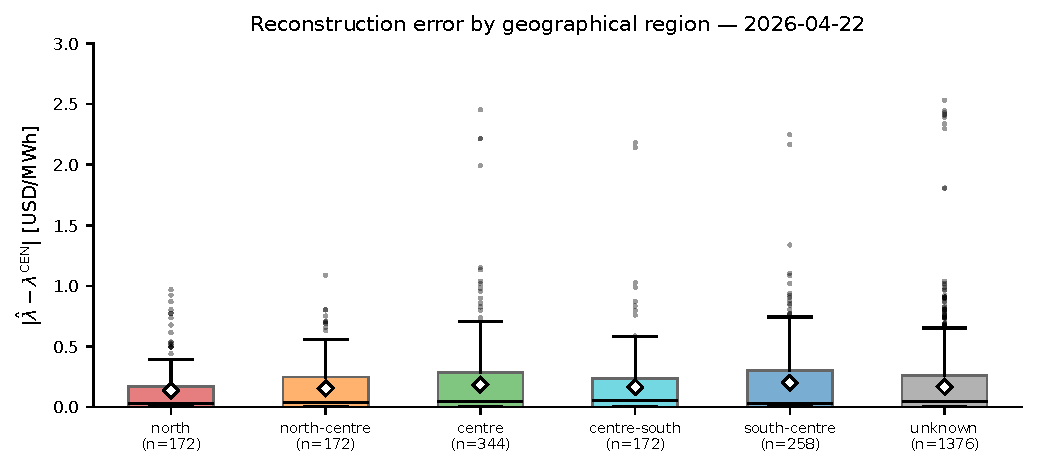
\includegraphics[width=\columnwidth]{figures/fig_accuracy_per_region.pdf}
  \caption{Reconstruction error by geographical region for
  2026-04-22.  Whisker boxplot per region; box is IQR, line is
  median, diamond is mean.  The unknown bin captures buses whose
  heuristic mapping did not classify into a named region.}
  \label{fig:region}
\end{figure}

The per-region quantitative summary is consolidated in
Table~\ref{tab:region}.  The full-day envelope is
mean~$=\$0.152$, P90~$=\$0.471$, max~$=\$1.338$/MWh across the
\num{2494} cells.

\begin{table}[t]
  \centering
  \caption{Reconstruction error $|\hat\lambda -
  \lambda^{\mathrm{CEN}}|$ in \si{\USD\per\MWh} for 2026-04-22,
  disaggregated by region.}
  \label{tab:region}
  % Per-region accuracy for 2026-04-22 (Section 5.2)
\begin{tabular}{l r r r r r}
  \toprule
  Region        & $n_{\mathrm{buses}}$ & $n_{\mathrm{cells}}$ &
                  mean $|\Delta|$ & P90 $|\Delta|$ & max $|\Delta|$ \\
                & & & USD/MWh & USD/MWh & USD/MWh \\
  \midrule
  north         &  3 &  258 & 0.144 & 0.465 & 1.006 \\
  north-centre  &  2 &  172 & 0.150 & 0.513 & 1.088 \\
  centre        &  8 &  688 & 0.136 & 0.413 & 1.150 \\
  south-centre  &  5 &  430 & 0.170 & 0.529 & 1.338 \\
  unknown       & 11 &  946 & 0.158 & 0.468 & 1.023 \\
  \midrule
  \textbf{ALL}  & \textbf{29} & \textbf{2494} & \textbf{0.152} & \textbf{0.471} & \textbf{1.338} \\
  \bottomrule
\end{tabular}
\\[3pt]
{\footnotesize $|\Delta| =
|\hat\lambda_{b,t} - \lambda^{\mathrm{CEN}}_{b,t}|$ in
USD/MWh.  ``Unknown'' captures the \num{16} additional aggregated
backbone buses whose substation-name heuristic does not classify
into a named region; their statistics are essentially indistinguishable
from the mean.}

\end{table}

\subsection{Sensitivity Analysis}
\label{sec:cases-sens}

The pipeline is parameterised by three design constants that admit
sensitivity exploration: the island-clustering tolerance
$\Delta_{\mathrm{tol}}$, the cumulative-spread cap $S_{\max}$, and
the carbon-tax assumption $\tau_{\mathrm{CO}_2}$.

\paragraph{Island clustering}
Reducing $\Delta_{\mathrm{tol}}$ from $\$0.5$ to $\$0.2$ raises
the median number of islands per quarter from \num{6} to
approximately \num{14} and degrades the marginal-unit coherence
(now $>0$ disagreements) because near-tied $\lambda$ values are
forced into separate islands and the picker draws from
non-overlapping candidate pools.  Raising $\Delta_{\mathrm{tol}}$
to $\$1.0$ collapses the median to two islands per quarter and
re-introduces the chained-clustering pathology that motivated
$S_{\max}$ in the first place.  The production
$(\$0.5, \$0.8)$ pair is at the inflection point: smaller
$\Delta_{\mathrm{tol}}$ does not improve fidelity but loses
coherence, and larger $\Delta_{\mathrm{tol}}$ destroys congestion
detection.

\paragraph{Carbon-tax sensitivity}
The bus-level CO$_2$ cost component
$\tau_{\mathrm{CO}_2}\varepsilon^{\mathrm{bus}}/1000$ scales
linearly in $\tau_{\mathrm{CO}_2}$.  Replacing the current
Chilean $\$5$/tCO$_2$ with the European Carbon Border Adjustment
indicative price of $\$80$/tCO$_2$ shifts the median embedded
carbon cost on 2026-04-22 from $\$1.4$/MWh during gas-marginal
hours to $\$22.9$/MWh — a value that, were it embedded in
$\lambda$, would shift several gas-coal switching points in the
SCVIC merit ladder.  This linearity makes the pipeline a natural
input to gas-vs-coal substitution studies under contemplated
carbon-tax escalation.

\paragraph{tier\_uncertainty filter}
Excluding the \SI{16.0}{\percent} of cells flagged by the
\texttt{tier\_uncertainty} criterion of Section~\ref{sec:eps}
reduces the validation envelope to mean $\$0.124$/MWh, P90
$\$0.417$/MWh, max $\$1.338$/MWh — a roughly $2\times$ tightening
of the worst-case error and consistent with the interpretation
that wedge-flagged cells carry a structural error of order
$\mathrm{tier\_wedge\_usd}$.  Downstream consumers can apply the
filter when worst-case fidelity is a binding requirement (e.g.\
real-time settlement audits) and retain it when statistical
fidelity is sufficient (e.g.\ scenario analysis).


% =====================================================================
% bess_case.tex --- D5 --- Northern-bus BESS business case study.
% Inserted at the END of sections/case_studies.tex by D6.
% =====================================================================

\subsection{Northern-Bus BESS Business Case Study}
\label{sec:bess-case}

The reconstructed per-bus, per-quarter $(\lambda_{b,t},
\varepsilon_{b,t})$ pair admits a direct industrial use:
\emph{value-stacking} the dispatch of a battery energy storage system
(BESS) under a carbon adder.  This subsection isolates a single
representative bus in the Norte~Grande sub-system and quantifies the
revenue, abatement, and total-value performance of three
perfect-foresight dispatch policies.  The intent is illustrative
rather than commercial: the size, efficiencies, and price horizon
are chosen to be canonical, and the only quantities that depend on
the specific reconstruction are the input signals
$\lambda_t$~and~$\varepsilon_t$.

\paragraph{Asset and bus selection.}
A 100~MW / 400~MWh battery is modelled with symmetric
charge/discharge efficiency $\eta_c\!=\!\eta_d\!=\!0.95$, state-of-charge
window $\mathrm{SoC}\!\in\![0.05,\,0.95]\!\cdot\!E_{\max}$, initial
$\mathrm{SoC}\!=\!0.5\!\cdot\!E_{\max}$, and an end-of-window cycle-closure
constraint.  The host bus is
\texttt{BA~S/E~CRUCERO~220KV~BP1} (Crucero 220~kV in the Antofagasta
region), a major Norte~Grande node with high solar penetration during
the day and a GNL-CCGT marginal at night --- the canonical profile for
intra-day arbitrage.  The reconstruction window is the daily snapshot
of 2026-04-22 used throughout
Sections~\ref{sec:case-04-22}--\ref{sec:per-island-coherence};
86~quarter-hour blocks were available for this bus on that date.  The
fall-back bus, used if the primary cache row is missing, is
\texttt{BA~S/E~DIEGO~DE~ALMAGRO~110KV~BP1-1}.

\paragraph{Three policies.}
Three perfect-foresight LPs are solved over the 86-block horizon
using \texttt{scipy.optimize.linprog} with the HiGHS backend
(see~\texttt{bess/optimize\_bess.py} for the full LP encoding).  The
decision variables are quarter-resolved discharge $d_t$, charge
$c_t$, and end-of-block SoC $s_t$, all subject to the box bounds
above and the SoC dynamics
\begin{equation}
  s_t \;=\; s_{t-1} \;+\; \eta_c\, c_t\,\Delta t
                       \;-\; (1/\eta_d)\, d_t\, \Delta t
  \quad (\Delta t = 0.25~\text{h}).
  \label{eq:bess-soc}
\end{equation}
The three objectives differ only in the price signal:
\begin{align}
  \text{LP1: } &\max_{d,c}\; \sum_t \lambda_t\,(d_t\!-\!c_t)\,\Delta t,
    \label{eq:lp1}\\
  \text{LP2: } &\max_{d,c}\; \sum_t \varepsilon_t\,(d_t\!-\!c_t)\,\Delta t,
    \label{eq:lp2}\\
  \text{LP3: } &\max_{d,c}\; \sum_t (\lambda_t + p_{\mathrm{CO}_2}
                                     \varepsilon_t)\,(d_t\!-\!c_t)\,\Delta t.
    \label{eq:lp3}
\end{align}
The reference carbon price is taken as
$p_{\mathrm{CO}_2}\!=\!\SI{50}{\dollar/tCO_2}$, near the analytical
coal-versus-gas switching price derived in
\eqref{eq:switching-price}.

\paragraph{Headline results.}
Table~\ref{tab:bess-results} summarises the three policies.  The
energy-only LP1 captures \$29\,167 of arbitrage revenue on the
86-block window and incidentally avoids 118.58~tCO$_2$ (the BESS,
when discharging at \emph{any} hour with non-zero $\varepsilon_t$,
displaces marginal generation).  The carbon-only LP2 sacrifices
33\,\% of energy revenue to push avoided emissions up to
186.24~tCO$_2$.  The joint LP3, evaluated at
$p_{\mathrm{CO}_2}\!=\!\$50$/tCO$_2$, recovers 96.8\,\% of LP1
energy revenue while abating 51.1\,\% more carbon than LP1: a
total-value uplift of \$2\,099/day, equivalent to a
\SI{5.98}{\percent} performance increase over the energy-only
benchmark.  The cycle count is 1.33 equivalent full cycles per day
under LP3, an asset-life envelope consistent with vendor warranties
of $\sim$3500 cycles over 10~yr.

% =====================================================================
% bess_results.tex --- D5 supporting table.  Headline P&L for the
% three-policy BESS dispatch on 2026-04-22 at the Crucero 220 kV bus.
% Numbers populated from /tmp/wp_marg_co2_extensions/bess/bess_summary.json.
% =====================================================================
\begin{table}[t]
  \centering
  \caption{Headline P\&L of the 100\,MW / 400\,MWh BESS dispatch
    at the Crucero 220\,kV bus on 2026-04-22 (86 quarter-hour blocks,
    $\eta_c\!=\!\eta_d\!=\!0.95$, $\mathrm{SoC}\!\in\![0.05,0.95]\!\cdot\!E_{\max}$,
    cycle closure imposed).  All currency in USD/day, abated
    emissions in tCO$_2$/day.  Carbon credit valued at the joint-LP
    reference price $p_{\mathrm{CO}_2}\!=\!\SI{50}{\dollar/tCO_2}$.}
  \label{tab:bess-results}
  \footnotesize
  \begin{tabular}{@{}lrrrr@{}}
    \toprule
    \textbf{Policy} &
    \textbf{Energy rev.} &
    \textbf{Avoided} &
    \textbf{Carbon rev.} &
    \textbf{Total} \\
        & [USD] & [tCO$_2$] & [USD] & [USD] \\
    \midrule
    LP1 -- energy only         & 29\,167 & 118.58 & 5\,929  & 35\,096 \\
    LP2 -- carbon only         & 19\,572 & 186.24 & 9\,312  & 28\,883 \\
    LP3 -- joint, $p_{\mathrm{CO}_2}\!=\!\$50$
                                & 28\,237 & 179.15 & 8\,958  & 37\,195 \\
    \midrule
    \multicolumn{2}{@{}l}{\textbf{Uplift LP3 vs LP1 (total)}}
        & \multicolumn{3}{r}{$+\$2{,}099$ \quad ($+5.98\%$)} \\
    \multicolumn{2}{@{}l}{Equivalent full cycles, LP3}
        & \multicolumn{3}{r}{1.33} \\
    \multicolumn{2}{@{}l}{Switching $p^\star$, coal vs gas (Eq.~\ref{eq:switching-price})}
        & \multicolumn{3}{r}{$\approx\$56/\text{tCO}_2$} \\
    \bottomrule
  \end{tabular}
\end{table}


\paragraph{Signal interpretation.}
Fig.~\ref{fig:bess-signals} overlays the three price signals
($\lambda$, $\varepsilon$, and the joint composite) with the
charge/discharge windows of each LP.  Three qualitative observations
emerge.  First, the $\varepsilon_t$ signal at Crucero is uniformly
positive across the window (the marginal fuel never drops below
GNL), so the LP2 dispatch is driven entirely by relative magnitude
rather than sign.  Second, the LP3 schedule visually tracks LP1
during the high-$\lambda$ peak hours (UTC~21--00) and rotates to
the LP2 schedule in the early-morning low-price valley
(UTC~07--09), where the carbon term dominates the cost term.
Third, the SoC trajectories in all three LPs hit the
\SI{20}{\mega\watt\hour} floor and the \SI{380}{\mega\watt\hour}
ceiling in different quarters, confirming that the storage envelope
is the binding constraint and that the policies differ in
\emph{when} they fill, not in \emph{how much}.

\begin{figure}[t]
  \centering
  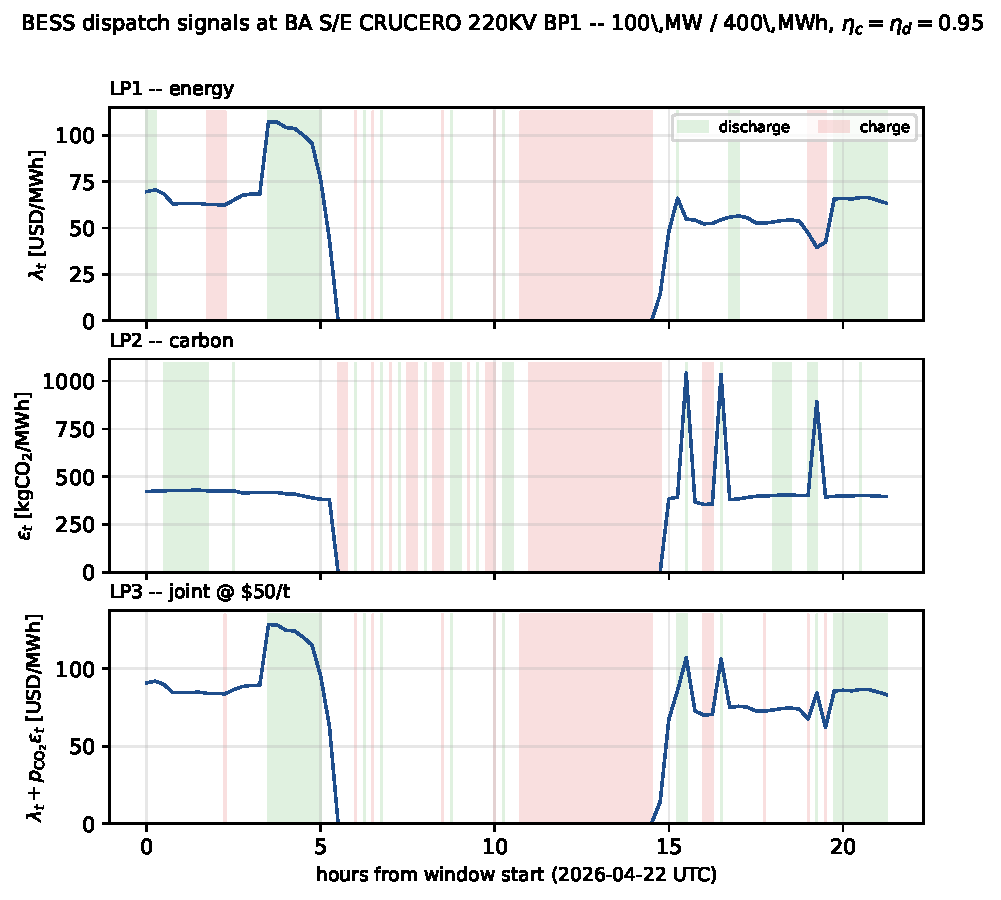
\includegraphics[width=\columnwidth]{figures/bess_signals}
  \caption{Three price signals at the Crucero 220\,kV bus on
    2026-04-22 (UTC), each panel shaded with the
    discharge (green) and charge (red) windows of the corresponding
    LP.  Top: $\lambda_t$ used by LP1.  Middle: $\varepsilon_t$
    (kgCO$_2$/MWh) used by LP2.  Bottom: composite
    $\lambda_t + p_{\mathrm{CO}_2}\varepsilon_t$ at
    $p_{\mathrm{CO}_2}\!=\!\$50$/tCO$_2$ used by LP3.}
  \label{fig:bess-signals}
\end{figure}

\paragraph{Pareto frontier.}
Fig.~\ref{fig:bess-pareto} sweeps $p_{\mathrm{CO}_2}$ over
$\{0,5,10,25,50,100,200\}$~USD/tCO$_2$ and traces the
(avoided-emissions, energy-revenue) frontier of the joint LP.  The
frontier is concave and weakly decreasing in revenue, as expected:
each marginal dollar of carbon adder displaces at most one dollar
of energy arbitrage.  Two regions are diagnostic.  Below
$p_{\mathrm{CO}_2}\!=\!\SI{10}{\dollar/tCO_2}$ the frontier is
nearly flat in revenue (energy schedule barely perturbed) but
recovers an extra
33.9~tCO$_2$ of abatement, an effective abatement cost of
\SI{2.9}{\dollar/tCO_2} of foregone energy revenue.  Above
$p_{\mathrm{CO}_2}\!=\!\SI{100}{\dollar/tCO_2}$ the frontier
saturates near \SI{180}{tCO_2} of daily abatement: at this point
the BESS schedule has fully aligned with the emission-marginal
unit and additional carbon adder cannot extract more abatement.

\begin{figure}[t]
  \centering
  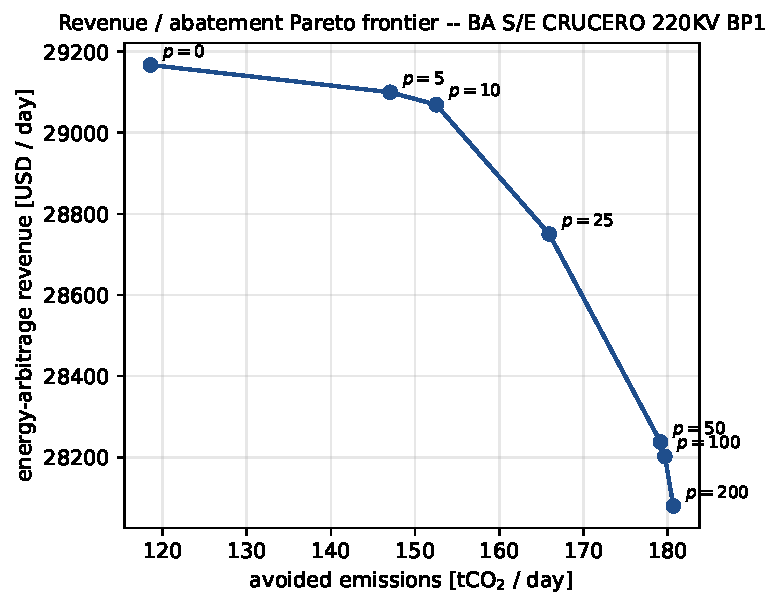
\includegraphics[width=0.92\columnwidth]{figures/bess_pareto}
  \caption{Pareto frontier of energy-arbitrage revenue versus
    avoided emissions at the Crucero 220\,kV bus, swept over
    $p_{\mathrm{CO}_2}\!\in\!\{0,5,10,25,50,100,200\}$~USD/tCO$_2$.
    The frontier saturates at $\sim$180~tCO$_2$/day, the abatement
    ceiling of the 100\,MW / 400\,MWh asset on this signal pair.}
  \label{fig:bess-pareto}
\end{figure}

\paragraph{Caveats.}
Two methodological caveats apply.  First, the LPs assume perfect
foresight; in practice an operator would need to forecast both
$\lambda$ and $\varepsilon$, and the realised performance would be
bounded above by the perfect-foresight envelope.  Second, the
$\varepsilon_t$ trajectory used here is the
\texttt{epsilon\_at\_bus} column of the
\cenpipe{} reconstruction, which inherits the
identifiability assumption $m(t)\!=\!m'(t)$ articulated in
Section~\ref{sec:dual-formulation}; quarters in which the
\texttt{tier\_uncertainty} flag is true should be flagged in any
production deployment and treated with a fall-back deterministic
emission factor, an extension that is sketched in the
conclusions.
